\documentclass[10pt,aspectratio=169]{beamer}
\usecolortheme{rose}
\usefonttheme{professionalfonts}
\usepackage[utf8]{inputenc}
\usepackage{fontspec}
\usepackage{minted}
\usepackage{unicode-math}
\usepackage{transparent}
\usepackage{tikz}
\usepackage{adjustbox}


\setsansfont[
UprightFont={* Light},
BoldFont={* Medium},
ItalicFont={* Light Italic}
]{Fira Sans}

\setmonofont{DejaVu Sans Mono}
\usepackage{hyperref}
% \setsansfont{Fira Sans}
% \setmathfont[Scale=MatchLowercase]{Fira Math}
\setmathfont{STIX Two Math}
\setmathrm{STIX Two Math}
\setboldmathrm{STIX Two Math}
% \usepackage{animate}
\usepackage[absolute,overlay]{textpos}
\usepackage{multimedia}
% \setmathfont{Fira Math Regular}
\title{\Large \bfseries Introduction to Logistic Regression}
\subtitle{\large CHE 358 Mock Lecture}
\author{\large Tian Tian}
\date{\large 22 June 2023}

\setbeamertemplate{footline}[frame number]
\beamertemplatenavigationsymbolsempty
\setbeamertemplate{itemize item}{\small $\bullet$}
\setbeamertemplate{itemize subitem}{\footnotesize $\bullet$}
\setbeamertemplate{itemize subsubitem}{\scriptsize $bullet$}

\begin{document} { \setbeamertemplate{footline}{} \frame{\titlepage} }


\begin{frame}[c]
  \frametitle{Perspective of Lecture}
  \begin{enumerate}
  \item The classification problem \vfill \item Logistic regression vs
    linear regression \vfill \item Fitting a logistic regression
    \vfill \item Case study: Li-ion battery failure \vfill \item
    Beyond logistic regression: neural networks
  \end{enumerate}
\end{frame}


\begin{frame}
  \frametitle{Linear Regression Recap}
  \begin{enumerate}
  \item Model Structure

    \vfill
    $y = f(x; \beta) = β_{0} + β_{1} x_{1} + β_{2} x_{x} + ... + β_{d}
    x_{d} + \epsilon \quad\quad \epsilon \sim N(0, \sigma^{2})$

    $x$ and $y$ are \textbf{continuous} variables.
    
    \vfill \item Assumptions

    \vfill
    \begin{itemize}
    \item \textbf{Linear} relation between $x$ and $y$
    \item \textbf{Independent} observations
    \item \textbf{Normal} distribution of error $\epsilon$
    \item \textbf{Constant} variance of error
    \end{itemize}


 
    \vfill \item Solving linear regression \vfill Least square fitting
    ${\displaystyle \hat{\beta} = \mathrm{argmin}\ S =
      \mathrm{argmin}\ \sum_{i=1}^{n} (y_{i} - f(x_{i}; \beta))^{2}}$
    
    \vfill \item Interpretation \vfill
    Coefficients $\beta$: how much $y$ change by one unit of $x$\\
    $R^{2}$: how well the model fits data
    
    
  \end{enumerate}

\end{frame}

\begin{frame}
  \frametitle{Categorical Response Variables}

  The assumption of \textbf{continuous} variables may not be true for
  many engineering problems.  If the output can only take a few
  allowed values, we call it a \textbf{categorical} response variable.

  \begin{figure}
    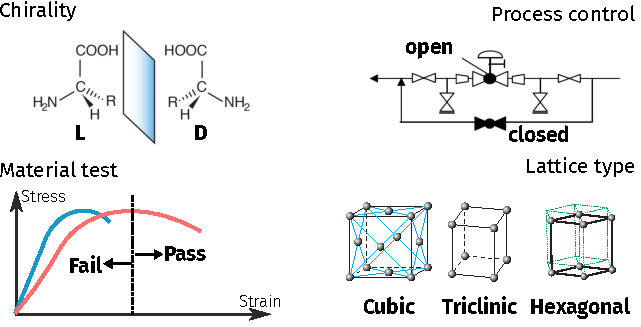
\includegraphics[width=0.85\textwidth]{images/categorical.pdf}
  \end{figure}

  % \begin{itemize}
  %   \vfill \item Diagnostics: a patient \textbf{obese} or
  %   \textbf{not obese} \vfill \item Decision: a valve to be turned
  %   \textbf{on} or \textbf{off} \vfill \item Data discretization:
  %   \textbf{pass} or \textbf{fail} a material strength test
  %   \vfill \item Describing types: \textbf{cubic},
  %   \textbf{hexagonal}, \textbf{triclinic} Bravais lattices, etc.

  % \end{itemize}

  % \vspace{2em}

\end{frame}



\begin{frame}
  \frametitle{Thought Experiment: the Cheater’s Coin}
  
  You're a casino owner who wishes to create a biased coin. Can you
  come up with a model to fit your measurements?

  \vfill
  \begin{columns}
    \begin{column}{0.25\textwidth}
      \begin{figure}[t]
        \centering 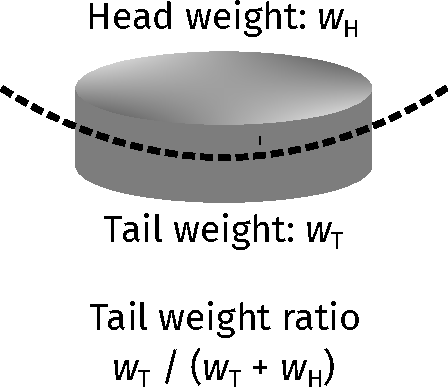
\includegraphics[width=\textwidth]{images/coin.pdf}
      \end{figure}
    \end{column}
    \begin{column}{0.75\textwidth}
      \movie{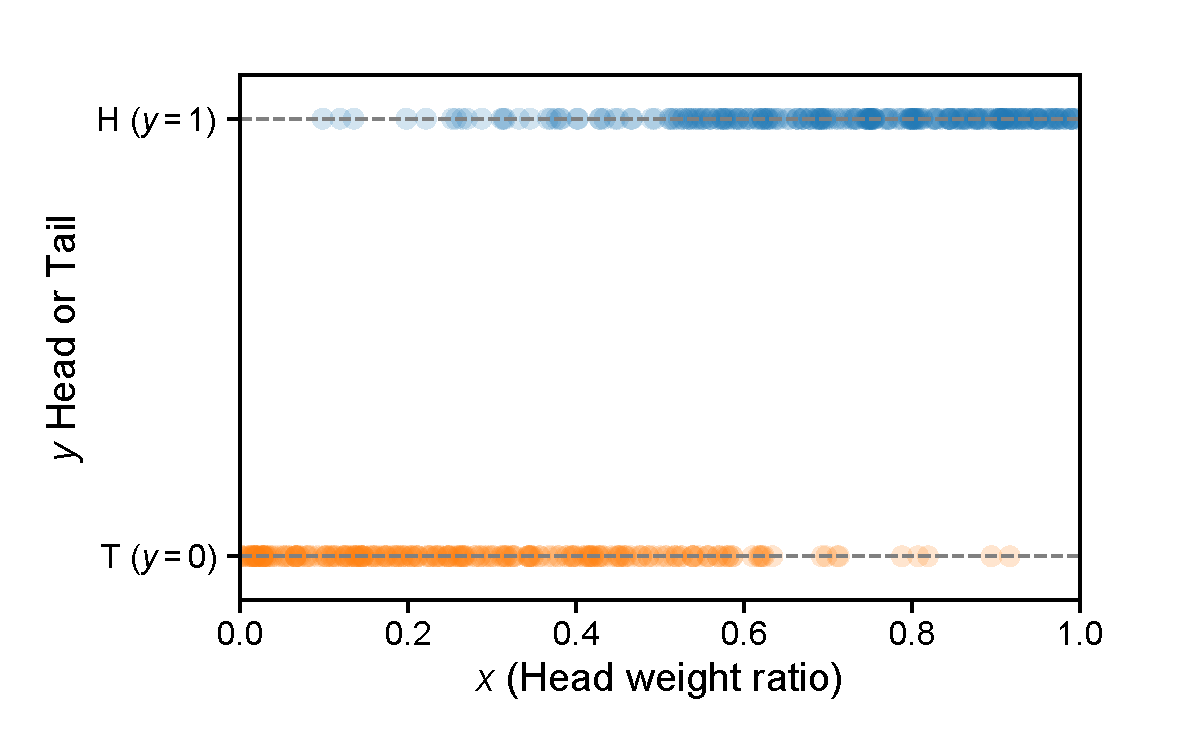
\includegraphics[width=\textwidth]{scripts/sample_coin_cover.pdf}}{scripts/animation.mov}
      % \begin{figure}[t]
      %   \animategraphics[width=\textwidth]{30}{scripts/animation-}{}{}
      %   \includegraphics[width=\textwidth]{animation.gif}
      % \end{figure}
    \end{column}
  \end{columns}

\end{frame}





\begin{frame}
  \frametitle{First Try: Linear Regression for Categorical Variables}

  Let's first try to use linear regression to fit the
  \textbf{probability} that our biased coin shows head. The
  probability function to fit is:
  \begin{equation*}
    y = p(x; \mathbb{\beta}) = \beta_{0} + \beta_{1} x
  \end{equation*}

  \vfill Our dataset
  \begin{itemize}
  \item Predictor (input) variable:
    $\mathbf{x} = \{x_{1}, x_{2}, \cdots, x_{n}\} \in \mathbb{R}^{(1,
      n)}$
  \item Response (predict) variable:
    $\mathbf{y} = \{y_{1}, y_{2}, \cdots, y_{n}\} \in \mathbb{R}^{(1,
      n)}$
  \item Parameter set:
    $\mathbf{\beta} = \{\beta_{0}, \beta_{1}\} \in \mathbb{R}^{(1,
      2)}$
  \end{itemize}

  \vfill Does linear regression makes sense?
  \begin{itemize}
  \item Range of predicted values?
  \item Distribution of residues?
  \item Are the predictions meaningful?
  \item Data extrapolation?
  \end{itemize}
\end{frame}


\begin{frame}
  \frametitle{Linear Regression Results}
  Let's compare the linear regression and analyze the residuals.
  \begin{figure}
    \centering %
    \hspace*{-0.05\textwidth}%
    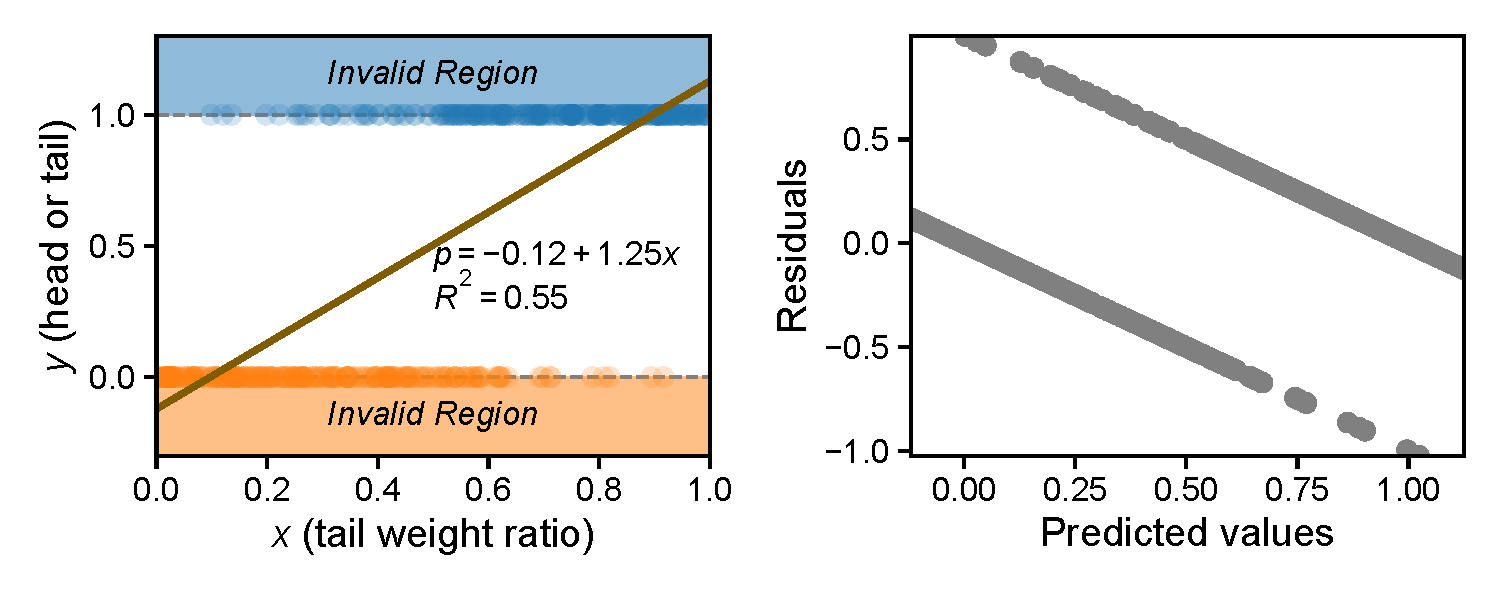
\includegraphics[width=1.10\textwidth]{scripts/coin_linear_combined.pdf}
  \end{figure}
\end{frame}
  

\begin{frame}
  \frametitle{Why Not Linear Regression?}
  As can be seen from previous example, linear regression is not
  suitable for predicting a dichotomous (binary) variable:

  \begin{enumerate}
    \vfill \item \textbf{Invalid predicted values}

    Probability should be between $(0, 1)$
  
    \vfill \item \textbf{Assumption of linearity violated}

    Residuals are not independent of observation (not normally
    distributed, not random)

  
    \vfill \item \textbf{Sensitive to data imbalance}

    If we have more "heavier-headed" coins sampled, the slope of
    linear regression will differ greatly.

    
    \vfill \item \textbf{Ambiguous definition of order and distance}

    Categorical variables (usually) do not have defined ordering or
    distance. Metrics like least square error do not make much sense
    (even worse for multi-class variables).
    
  \end{enumerate}
\end{frame}

\begin{frame}
  \frametitle{Second Try: Non-Linear Regression}
  % Making the probability function $p(x; \beta)$ non-linear may solve
  % the problem!  But what will its expression be?

  % \vfill
  
  Recall: for binary outcome $y_{i} \in (0, 1)$, $p(x_{i}; \beta)$
  means the probability of that the outcome $y_{i}=1$, given the input
  $x_{i}$ and parameters $\beta$:
  \begin{equation*}
    p(x_{i}; \beta) = \mathrm{Prob}(y_{i}=1 | x=x_{i}; \beta)
  \end{equation*}

  \vspace{1em}

  We could infer some properties of a non-linear $p$:
  \begin{enumerate}
  \item \textbf{Range}:

    $p$ maps $x \in \mathbb{R}$ to $y \in (0, 1)$.
    
  \item \textbf{Linearization}:

    We want $p$ to be ``linearizable'', i.e. to separate $x$ and
    $\beta$ to L.H.S via function inversion:

    \begin{equation*}
      p^{-1} = \mathrm{Inversion}(p) = \beta_{0} + \beta_{1} x_{i}
    \end{equation*}

  \item \textbf{Continuity}:

    To satisfy the linearization, $p$ should be continuous and
    monotonic in $\mathbb{R}$ (why?)
    
  \end{enumerate}
  
\end{frame}

\begin{frame}
  \frametitle{Candidates for Non-Linear Regression}

  A series of S-shaped (sigmoid) functions may meet our
  criteria. Let's check their plots in 1D.
  \vfill
  \begin{figure}[t]
    \only<1>{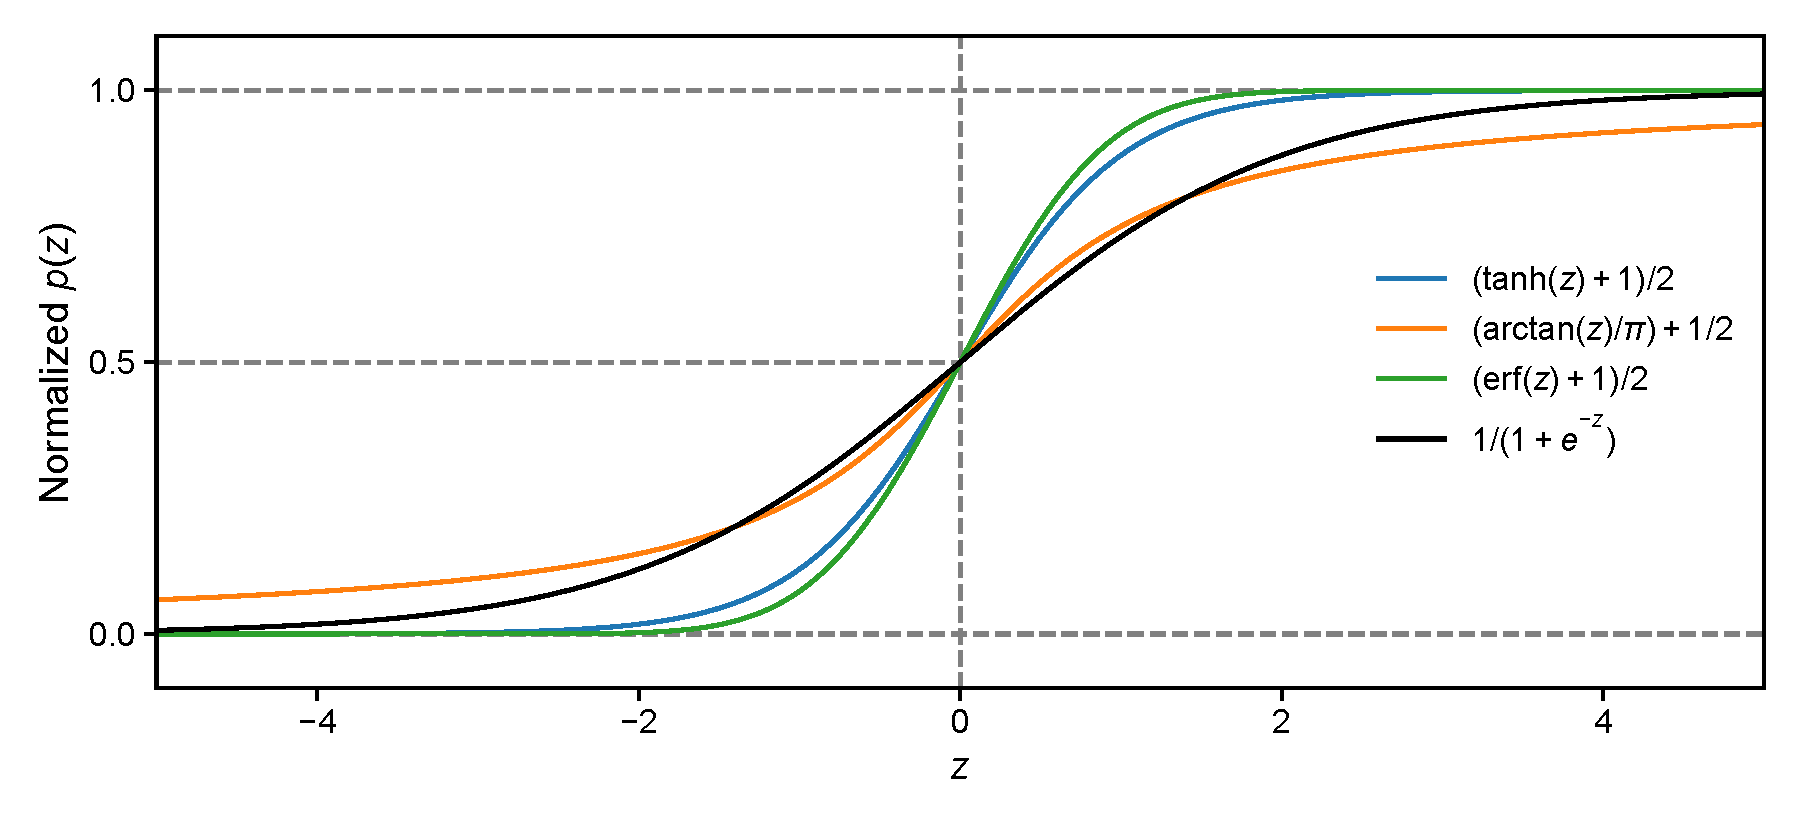
\includegraphics[width=1.\textwidth]{scripts/sigmoid_funs.pdf}}
    \only<2>{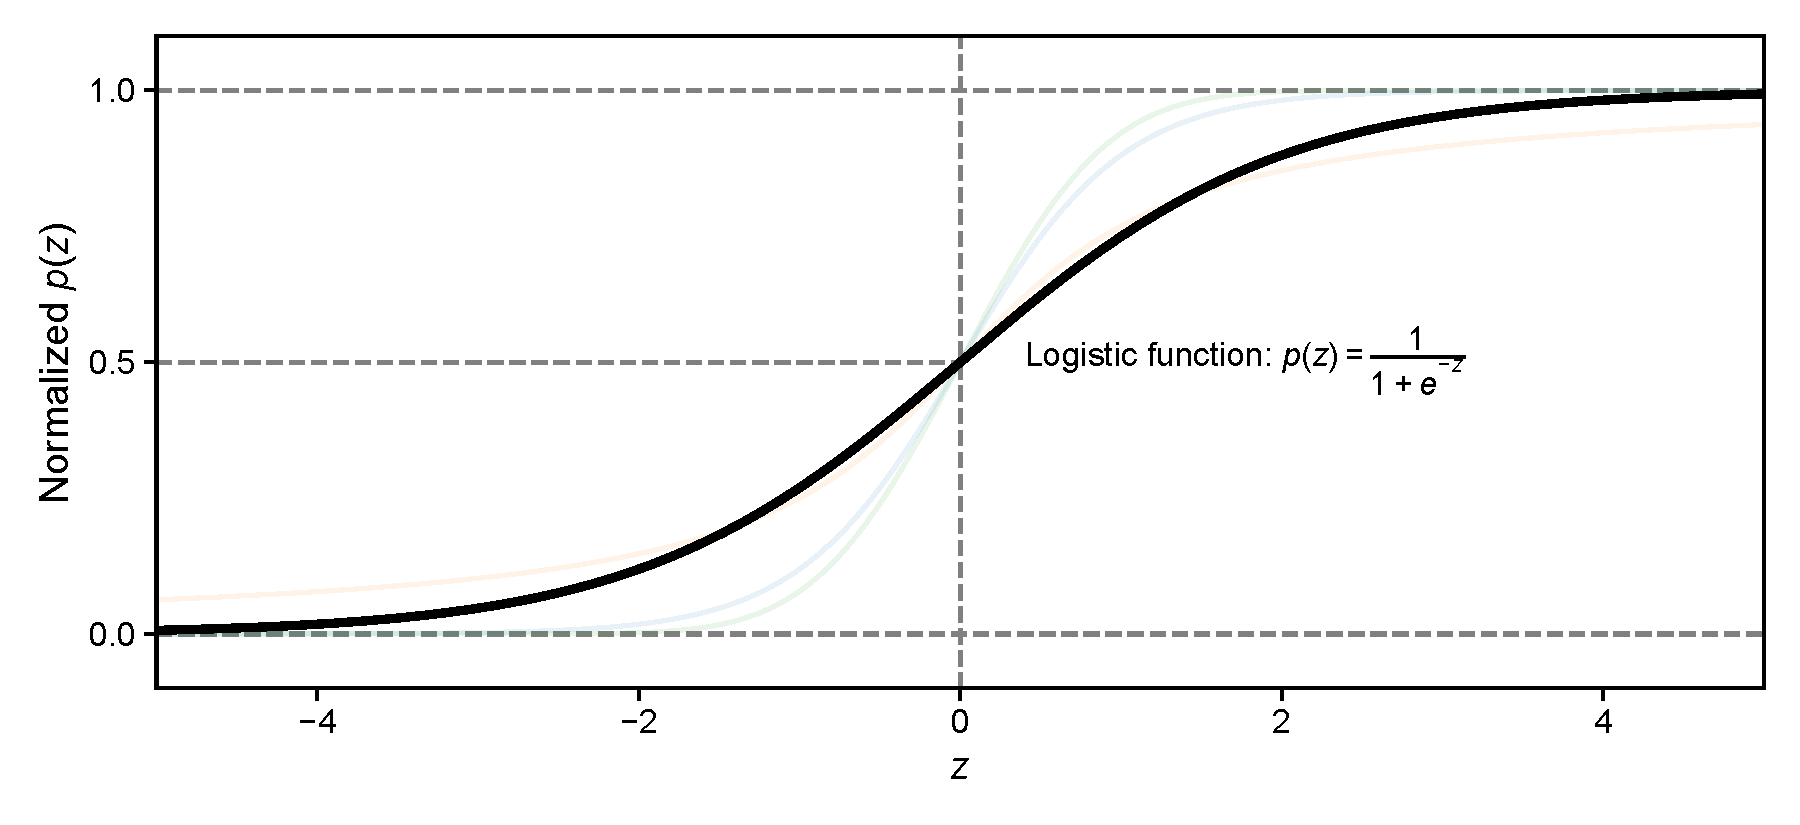
\includegraphics[width=1.\textwidth]{scripts/sigmoid_funs_emphasize_logistic.pdf}}
  \end{figure}
\end{frame}

\begin{frame}
  \frametitle{The Logistic Function: Properties}
  
  In 1D form, the sigmoid function $p(z) = 1/(1 + \mathrm{exp}(-z))$
  is called the \textbf{logistic function} \let\thefootnote\relax\footnotetext{{\scriptsize
      In machine learning, \textit{sigmoid} function explicitly means
      logistic function.}}.
    %
  The process of fitting binary dataset is referred to as
  \textbf{logistic regression}.

  \begin{columns}[T]
    \begin{column}{0.4\textwidth}
      \begin{enumerate}
      \vfill \item Asymptotic behavior
          
        $\mathrm{lim}_{z\to\infty} p(z) = 1$
          
        $\mathrm{lim}_{z\to-\infty} p(z) = 0$
          
      \vfill \item Symmetry

        $p(z) = 1 - p(-z)$
          
      \vfill \item Point of inflection

        $p(0) = \frac{1}{2}$
          
      \vfill \item Inverse function

        $p^{-1} = \mathrm{log}(\frac{p}{1 - p})$

      \vfill \item 1st and 2nd Derivatives

        $p^{'}(z) = p(z)(1 - p(z))$

        $p^{''}(z) = p'(z)(1 - 2 p(z))$
      \end{enumerate}
    \end{column}

    \begin{column}{0.5\textwidth}

        \begin{figure}[t]%
          \hspace*{-0.1\textwidth}%
          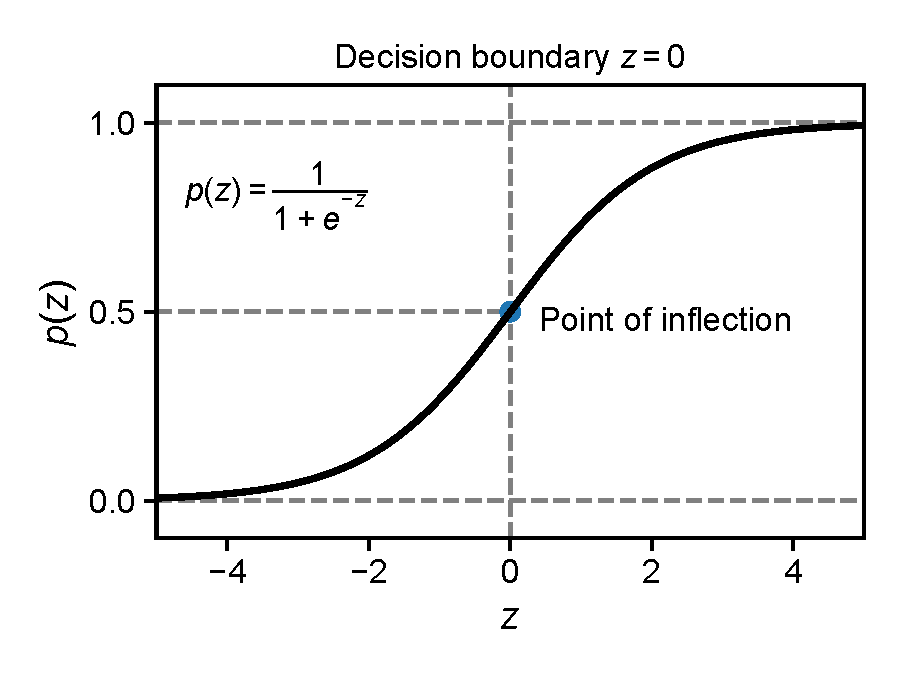
\includegraphics[width=1.2\textwidth]{scripts/logistic_fun_alone.pdf}
        \end{figure}
        
      \end{column}
      
    \end{columns}
  \end{frame}

  \begin{frame}
    \frametitle{Linear Regression: Formal Definition (1D)}
    Problem: for a given dataset
    $\mathbb{D} = \{(x_{i}, y_{i}), \cdots, (x_{n}, y_{n})\}$,
    estimate the probability that the input $x$ belongs to one of the
    binary output $y \in (0, 1)$, where $x_{i} \in \mathbb{R}^{1}$.

    \vfill Model: we use a linear combination of the input variable
    $x$ with parameter $\beta$ to construct the logistic function:
    \begin{equation*}
      p(x; \beta) = \dfrac{1}{1 + e^{-(\beta_{0} + \beta_{1} x)}} = \dfrac{e^{\beta_{0} + \beta_{1} x}}{1 + e^{\beta_{0} + \beta_{1} x}}
    \end{equation*}

    \vfill Linearization: recall the inverse function of the logistic
    function
    \begin{equation*}
      p^{-1}(x; \beta) = \mathrm{Logit}(p) = \mathrm{log} (\dfrac{p}{1 - p} ) = \beta_{0} + \beta_{1} x
    \end{equation*}

    $p^{-1}$ is called the \textbf{Logit} function, measuring the
    log-odds (i.e. probability ratio between a head and tail). %
    \vfill%
    \textbf{Question: can be directly use the Logit function form to perform a
    logistic regression?}
  
  \end{frame}

  \begin{frame}
    \frametitle{Fitting by Logistic Function: the Maximum Likelihood
      Estimation}

    A common approach to solve logistic regression is to maximize the
    \textbf{likelihood function} $\mathscr{L}(\beta|\mathbb{D})$ of the
    logistic function by varying the parameter set $\beta$.

    The logistic regression problem is solved by find:

    \begin{equation*}
      \hat{\beta} = \mathrm{argmax}\ \mathscr{L}(\beta|\mathbb{D})
    \end{equation*}
    
    \begin{figure}[t] %
       \vspace{-2em}%
           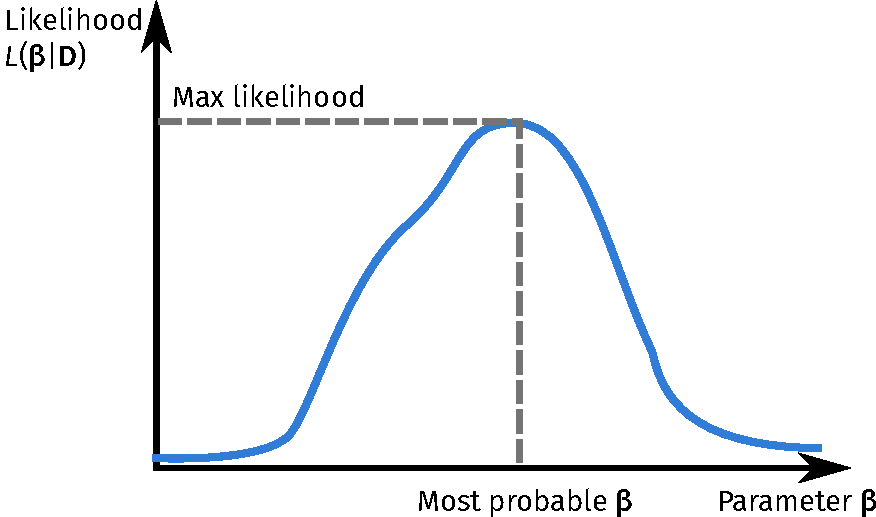
\includegraphics[width=0.7\textwidth]{images/likelihood.pdf}
         \end{figure}

    
       \end{frame}


       \begin{frame}
         \frametitle{The Likelihood of Logistic Function}

         The likelihood $L(\beta)$ of logistic functions follows the
         Bernoulli distribution\let\thefootnote\relax%
         \footnotetext{\scriptsize Montgomery \& Runger, Applied Statistics \& Probability for Engineers, 6th Ed, Chapter 7}.%
         Assume for any datum 
         %
         $(x_{i}, y_{i})$, $p_{i} = p(x_{i}; \beta)$, we have:

        \begin{equation*}
          \mathscr{L}(\beta|\mathbb{D}) = \prod_{i=1}^{n} p_{i}^{y_{i}} (1 - p_{i})^{1-y_{i}}
        \end{equation*}

        The log-loss likelihood $\mathscr{l}$ is used more frequently:
        \begin{equation*}
          \mathscr{l}(\beta|\mathbb{D}) = -\mathrm{log} L(\beta|\mathbb{D}) = \sum_{i=1}^{n} -y_{i} \mathrm{log}p_{i} -  (1 - y_{i}) \mathrm{log}(1 - p_{i})
        \end{equation*}
        
        
        $\mathscr{l}(\beta|\mathbb{D})$ is the actual \textbf{cost
          function} of logistic regression.  \vfill
        
        Now we just need to solve the optimal parameter set
        $\hat{\beta} = \mathrm{argmin}\
        \mathscr{l}(\beta|\mathbb{D})$.
        
      \end{frame}


      \begin{frame}
        \frametitle{Numerical Optimization of the Cost Function:
          Gradient Descent}
        The likelihood function \textbf{does not} have a closed-form
        solution and the minimal value of $l(\beta)$ has to be solved
        numerically.

        \vfill Algorithm: for each parameter $\beta_{j}$ ($j=0, 1$),
        we pick the initial guess $\beta_{j}^{0}$, compute
        $l(\beta|\mathbb{D})$ and the first derivative
        $\partial l/\partial \beta_{j}$. We then iteratively update
        $\beta_{j}$ by the Newton's method between steps $s$ and
        $s+1$:

        \begin{align*}
          \beta_{0}^{s+1} &= \beta_{0}^{s} - \alpha^{s} \dfrac{l(\beta^{s})}{\partial l/\partial \beta_{0}} \\
          \beta_{1}^{s+1} &= \beta_{1}^{s} - \alpha^{s} \dfrac{l(\beta^{s})}{\partial l/\partial \beta_{1}}
        \end{align*}

        The parameter $\alpha^{s}$ is called the \textbf{learning
          rate} (at step $s$), an important hyper-parameter in machine
        learning.

        \vfill
        \textbf{Question: where are the data points $(x_{i}, y_{i})$ in
        the above equation?}

      \end{frame}

      \begin{frame}
        \frametitle{Gradients of Logistic Regression}
        %
        \begin{tikzpicture}[remember picture,overlay]
\node[anchor=north east,yshift=-0.1cm] at (current page.north east) {\textcolor{magenta}{\textbf{In-depth Analysis}}};
\end{tikzpicture}
%
        The logistic function is a
        perfect candidate for gradient-based optimization due to the
        neat form of gradients.

        \vfill We can rewrite the cost function
        $\mathscr{l}(\beta|\mathbb{D})$ of logistic function as:

        \begin{equation*}
          \mathscr{l}(\beta|\mathbb{D}) = \sum_{i=1}^{n}  -\log (1 - p_{i}) - y_{i} (\beta_{0} + \beta_{1}x_{i})
        \end{equation*}

        Then the first partial derivatives are:
        \begin{align*}
          \dfrac{\partial \mathscr{l}}{\partial \beta_{0}}
          &= -\sum_{i=1}^{n} \left[ -\frac{1}{1 + e^{-(\beta_{0} + \beta_{1} x)}} + y_{i} \right] = \sum_{i=1}^{n} (p_{i} - y_{i})\\
          \dfrac{\partial \mathscr{l}}{\partial \beta_{1}}
          &= -\sum_{i=1}^{n} \left[ -\frac{1}{1 + e^{-(\beta_{0} + \beta_{1} x)}}x_{i} + y_{i}x_{i} \right]= \sum_{i=1}^{n} (p_{i} - y_{i})x_{i}
        \end{align*}
        
        \vfill In practice, other methods like the
        Broyden–Fletcher–Goldfarb–Shanno (BFGS) algorithm are used
        instead of Newton's method.

        
      \end{frame}

      \begin{frame}
        \frametitle{Logistic Regression Demo: Cheater’s Coin}
        \begin{columns}[T]
          \begin{column}{0.45\textwidth}
            Logistic regression using Python's scikit-learn library:
            
            \inputminted[fontsize=\scriptsize]{python}{sample_lr_coin.py}
          \end{column}

          \begin{column}{0.55\textwidth}
            \begin{figure}[t]%
              \hspace*{-0.1\textwidth}%
              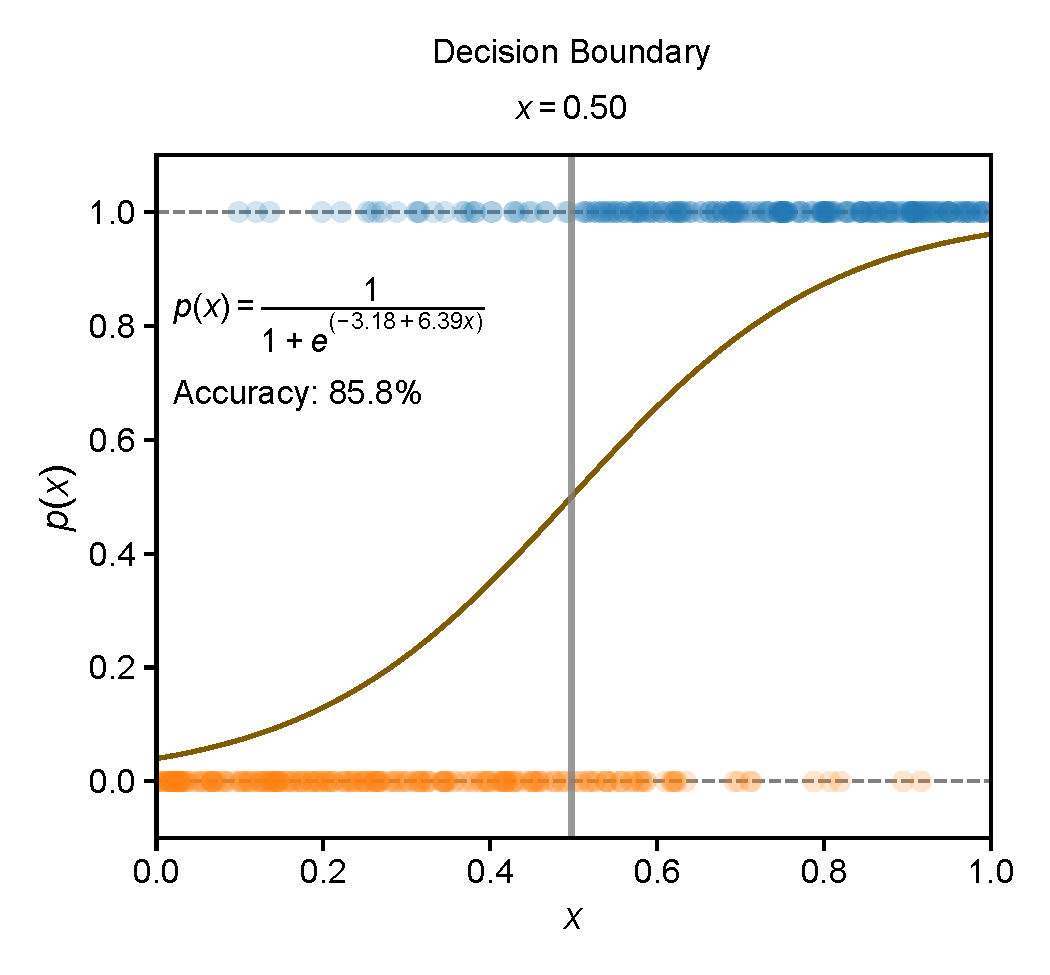
\includegraphics[width=1.20\textwidth]{scripts/coin_fit_lr.pdf}
            \end{figure}
          \end{column}
        \end{columns}

        Do you spot any issues?
      \end{frame}

     

      \begin{frame}
        \frametitle{Caveat: Regularization}
        
        The naive logistic regression may work poorly on some
        datasets.  Let's modify the coin example a bit. This time, the
        coin will always ends in head when $x > 0.5$, and tail if
        $x < 0.5$. Which model is correct?  \textbf{TODO: change the
          plot axis and shape}

        \begin{figure}[t]
          \vspace{-1em}
          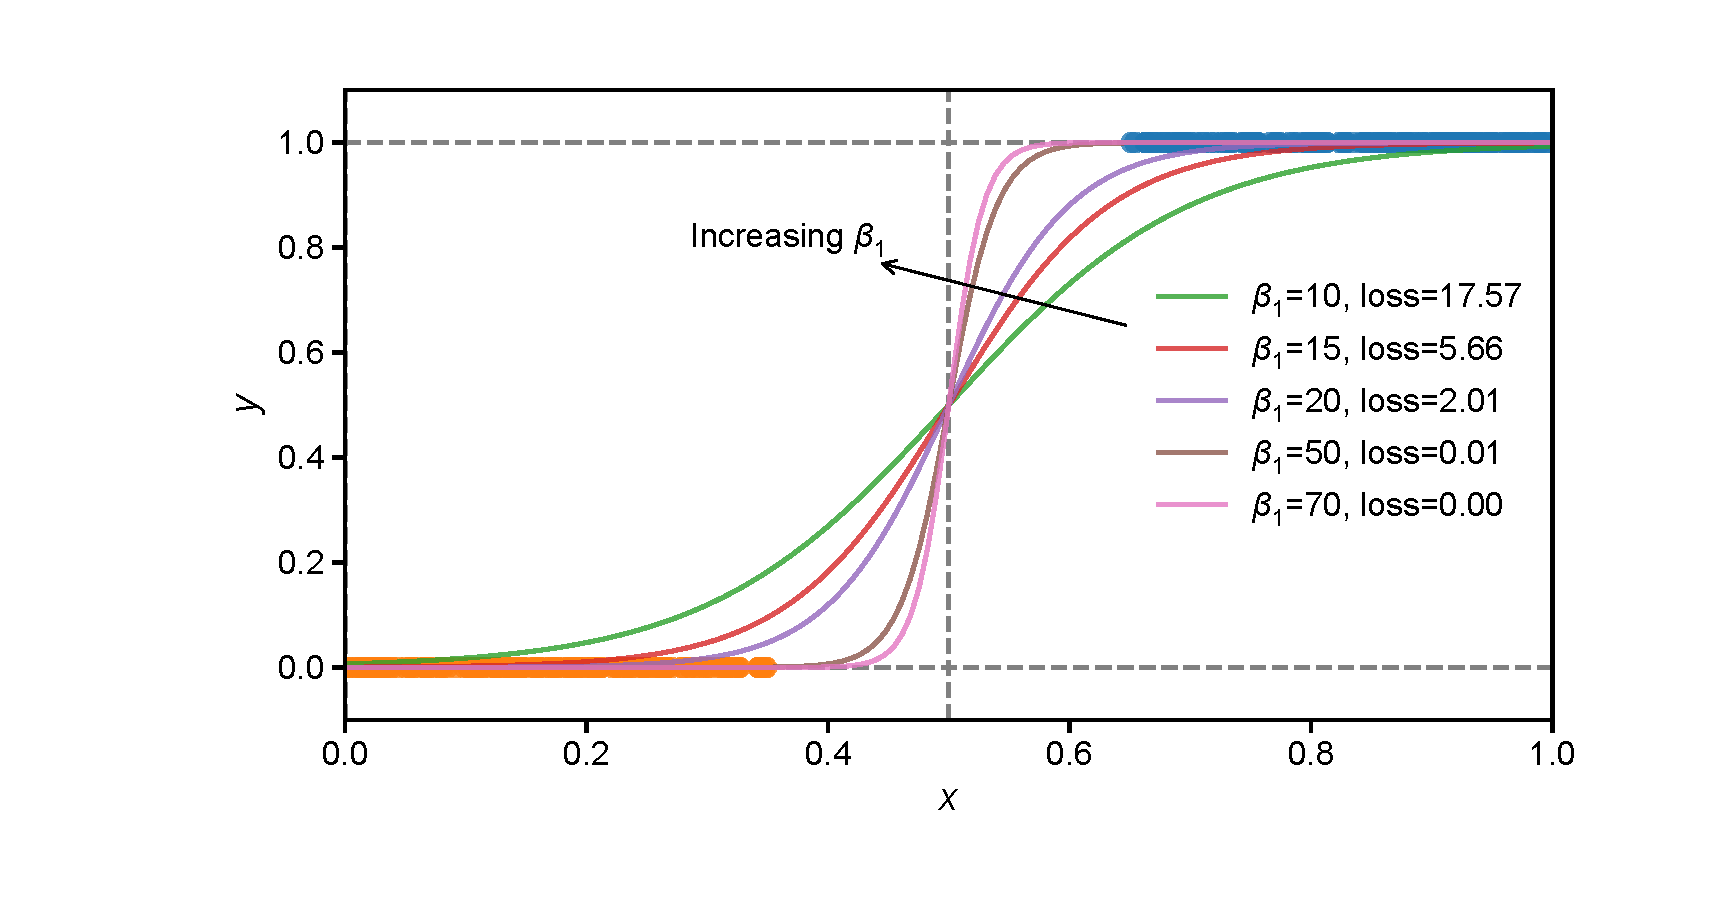
\includegraphics[width=0.90\textwidth]{scripts/perfect_sep.pdf}
        \end{figure}
        
      \end{frame}

      \begin{frame}
        \frametitle{Regularization (1)}

        The naive logistic regression may lead to
        \textbf{over-fitting}.  We can add additional penalty terms
        $P(\beta)$ to our cost function to avoid large coefficient
        $\beta$ (weights). Two commonly used regularization methods in
        statistics and machine learning are
        \let\thefootnote\relax\footnotetext{ The choice of L1 or L2
          depends on the problem.}:

        \begin{itemize}
        \item L1 (lasso) regularization
          \begin{equation*}
            P(\beta) = \sum_{j=0}^{d} |\beta_{j}| 
          \end{equation*}

          
        \item L2 (ridge) regularization
          \begin{equation*}
            P(\beta) = \sum_{j=0}^{d} \beta_{j}^{2}
          \end{equation*}
        \end{itemize}

        The full cost function $C(\beta)$ for logistic regression is
        then:
        \begin{equation*}
          C(\beta) = \mathscr{l}(\beta) + \lambda P(\beta)
        \end{equation*}
        where $\lambda$ is the strength of regularization penalty.
      \end{frame}

      \begin{frame}
        \frametitle{Regularization (2)}
        Let's see how regularization helps in the previous case:

        \begin{figure}[t]
          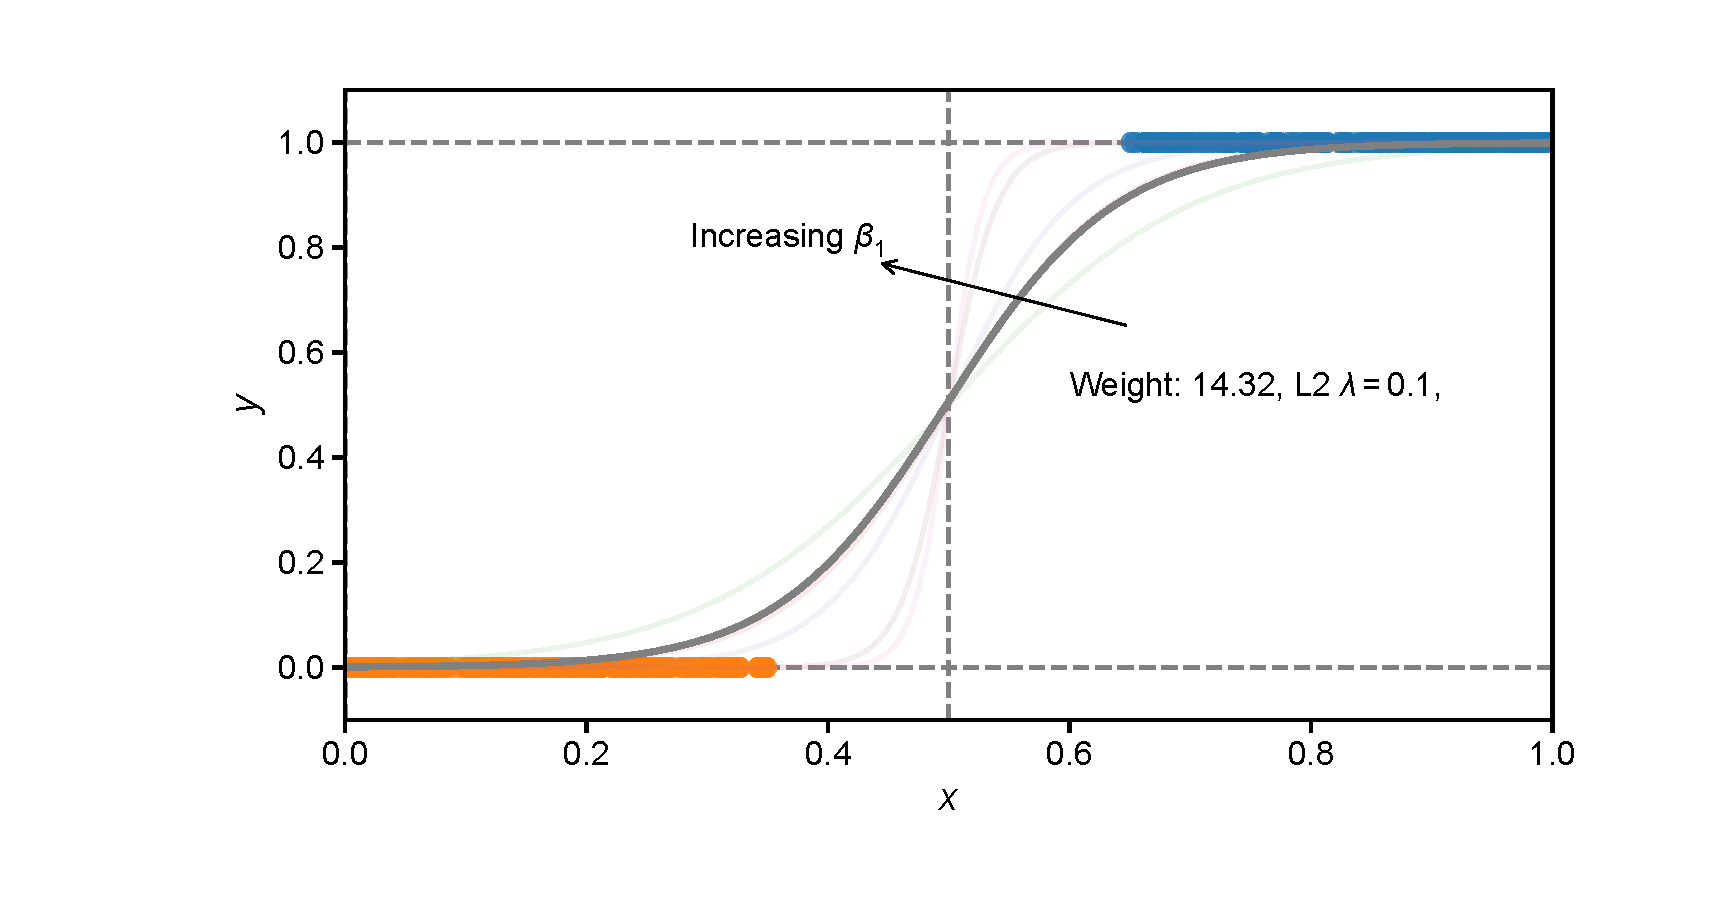
\includegraphics[width=0.95\textwidth]{scripts/perfect_sep_reg.pdf}
        \end{figure}
      \end{frame}

      \begin{frame}
        \frametitle{How Do We Measure the Performance?}
        \begin{enumerate}
          \vfill \item \textbf{Cost function}
          $\mathscr{l}(\beta | \mathbb{D})$ can be a convenient
          measurement when rank different models.
          
          \vfill \item \textbf{Classification accuracy}
          
          Accuracy =
          $\dfrac{N(\mathrm{correctly\ predicted})}{n} \times 100\%$
          
          \vfill \item \textbf{Confusion matrix}

          Similar to accuracy, but with percentage of true positive
          (TP), true negative (TN), false positive (FP), false
          negative (FN).
          
          \vfill \item \textbf{(Pseudo)} $R^{2}$

          Unlike ordinary least square, logistic regression does not
          have uniquely defined $R^{2}$, although some pseudo-$R^{2}$
          metrics have been proposed.
        \end{enumerate}
        
      \end{frame}

      \begin{frame}
        \frametitle{Interpret the Logistic Regression Results}
        Recall the linearization of the logistic function in 1D:

        \begin{equation*}
          \log \left(\frac{p}{1 - p}\right) = \beta_{0} + \beta_{1}x
        \end{equation*}

        There are some intuitions for the coefficients:
        \begin{enumerate}
          \vfill \item Increase $x$ by 1 amplifies the odd ratio by
          $e^{\beta_{1}}$ \vfill \item At
          $x = - \dfrac{\beta_{0}}{\beta_{1}}$, the odd ratio is 1
          \vfill \item Positive $\beta_{1}$: the probability of
          predicted class ($y=1$) increases with larger $x$
          \vfill \item Negative $\beta_{1}$: the probability of
          predicted class ($y=1$) decreases with larger $x$
        \end{enumerate}
      \end{frame}

      \begin{frame}
        \frametitle{Logistic Regression in Higher Dimensions}

        It is straightforward to extend the logistic regression if
        input variable $\mathbf{x} \in \mathbb{R}^{d}$.  \vfill
        \textbf{Model}:
        \begin{align*}
          p(\mathbf{x}; \beta) &= \dfrac{1}{1 + e^{-(\beta_{0} + \sum_{j=1}^{d} \beta_{d} x_{d})}} = \dfrac{1}{1 + \exp(- \beta^{T} \mathbf{X})}
        \end{align*}
        here $\mathbf{X} = {1, x_{0}, x_{1}, \cdots, x_{d}}$.

        \vfill \textbf{Likelihood function}:
        \begin{align*}
          \mathscr{l}(\beta; \mathbb{D}) = -\sum_{i=1}^{n}\left[y_{i} \log p_{i} + (1 - y_{i})\log (1 - p_{i}) \right] 
        \end{align*}

        \vfill \textbf{Gradient}:
        \begin{align*}
          \frac{\partial \mathscr{l}}{\partial \beta_{j}}
          &= -\sum_{i=1}^{n} -\frac{1}{1 + \exp(-\beta^{T} \mathbf{X}_{i})} x_{ij} + y_{i}x_{ij} \\
          &= \sum_{i=1}^{n} (p_{i} - y_{i})x_{ij}
        \end{align*}
        where $x_{ij}$ is the $j$-th component in $i$-th datum.
        
      \end{frame}

      \begin{frame}
        \frametitle{Real-World Example: Li-ion Battery Failure (1)}

        Can you predict if a lithium-ion battery in EV will fail from
        measurements\let\thefootnote\relax\footnote{{\tiny Zhao et
            al. \textit{iScience} \textbf{25}, 104172}}?

        \begin{figure}[t]
          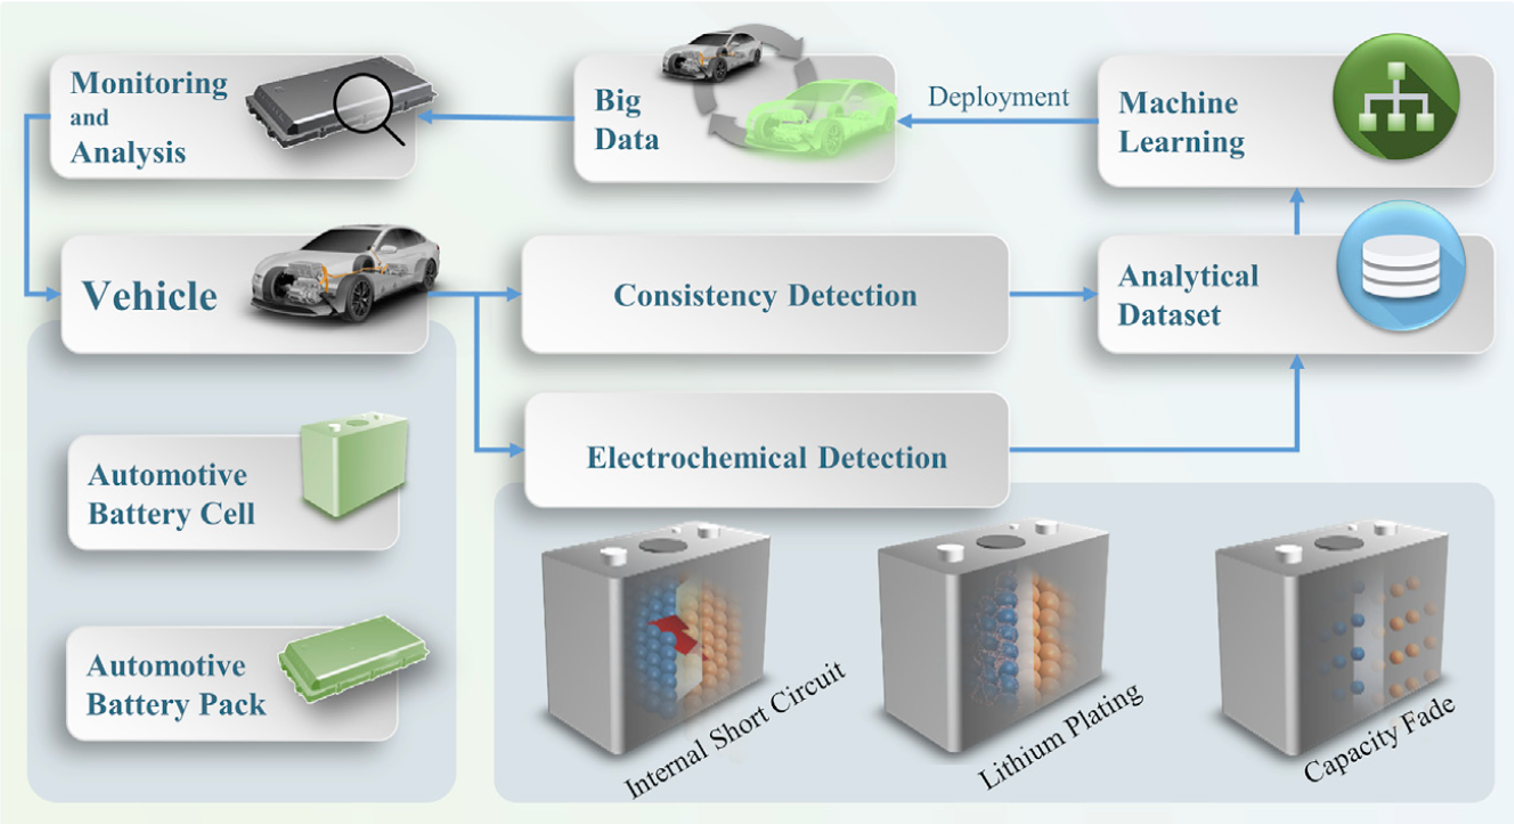
\includegraphics[width=0.9\linewidth]{images/battery_1.png}
        \end{figure}

      \end{frame}

      \begin{frame}
        \frametitle{Real-World Example: Li-ion Battery Failure (2)}
        Battery failure
        dataset. \let\thefootnote\relax\footnote{{\tiny Zhao et
            al. \textit{iScience} \textbf{25}, 104172}}.

        \begin{figure}[t]
          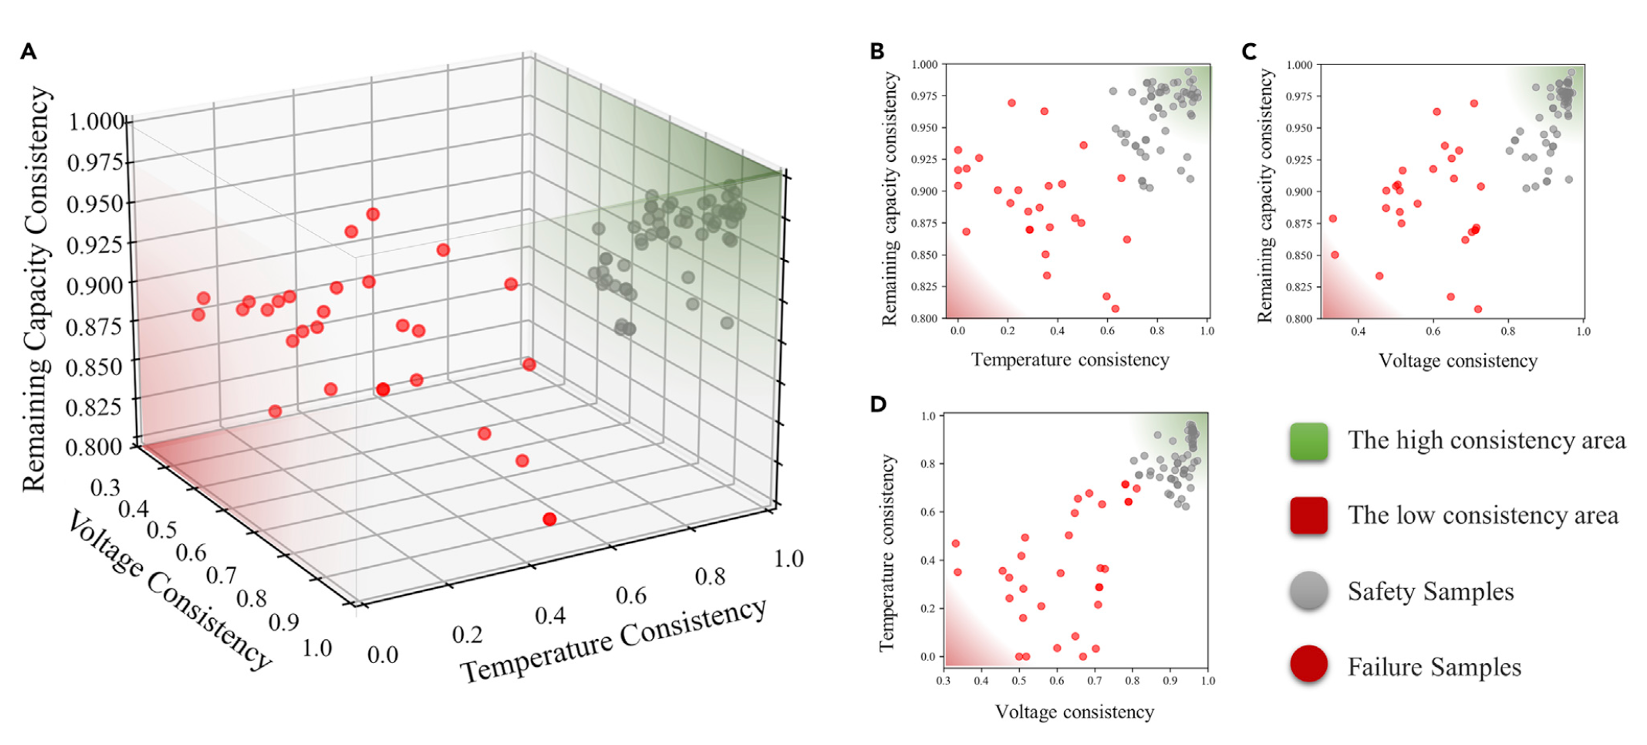
\includegraphics[width=1.0\linewidth]{images/battery_2.png}
        \end{figure}
      \end{frame}

      \begin{frame}
        \frametitle{Real-World Example: Li-ion Battery Failure
          (3)\let\thefootnote\relax\footnote{{\tiny See course
              material
              \url{https://github.com/alchem0x2A/uoa_che358_mock}}}}

        \begin{itemize}
        \item Step 1: Dataset split (train / test)

          Rule of thumb: 80/20 or 70/30 rule
          
        \item Step 2: Create a logistic regression model

          See our example in coin dataset
          
        \item Step 3: Hyper-parameter tuning

          Some hyper-parameters (e.g. regularization) may affect model
          performance beyond $\beta$
          
        \item Step 4: Model accuracy test

          Additional dataset or cross-validation
        \end{itemize}
        
        
      \end{frame}

      \begin{frame}
        \frametitle{Real-World Example: Li-ion Battery Failure
          (4)\let\thefootnote\relax\footnote{{\tiny See course
              material
              \url{https://github.com/alchem0x2A/uoa_che358_mock}}}}

        \textbf{TBD}
        
        
      \end{frame}

      \begin{frame}
        \frametitle{Advanced Topic: Logistic Regression to Neural
          Network (1)}
        In machine learning, the logistic regression can be viewed as
        a single perceptron (neuron).

        \begin{figure}[t]
          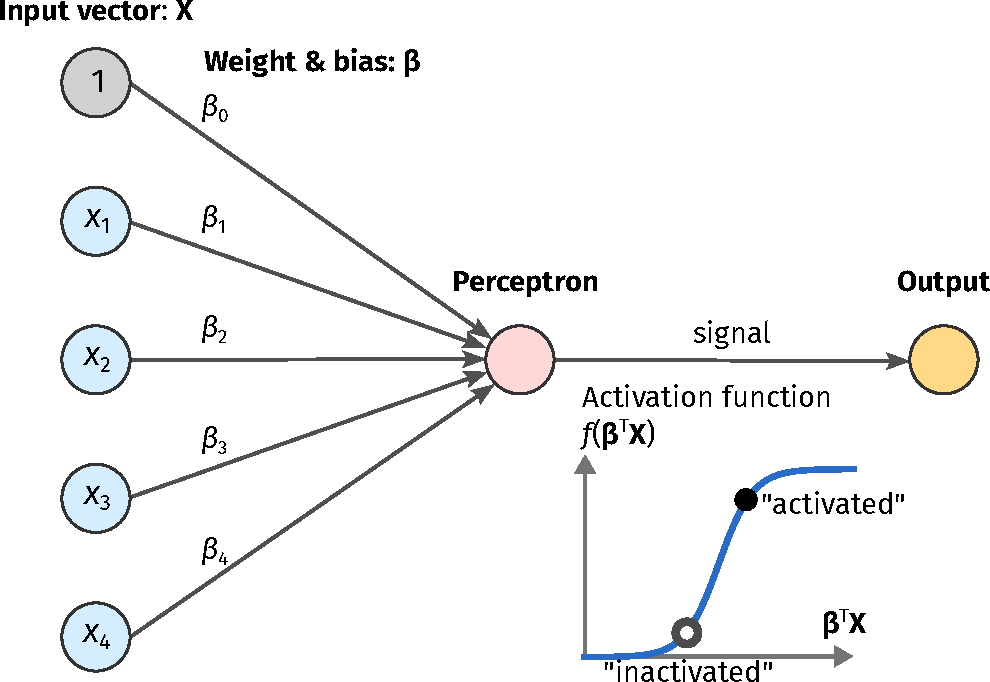
\includegraphics[width=0.65\linewidth]{images/nn-1.pdf}
        \end{figure}

        
      \end{frame}

      \begin{frame}
        \frametitle{Advanced Topic: Logistic Regression to Neural
          Network (2)}
        We can extend the single ``logistic perceptron'' to a complex
        ``neural network'' (NN).

        \begin{figure}[t]
          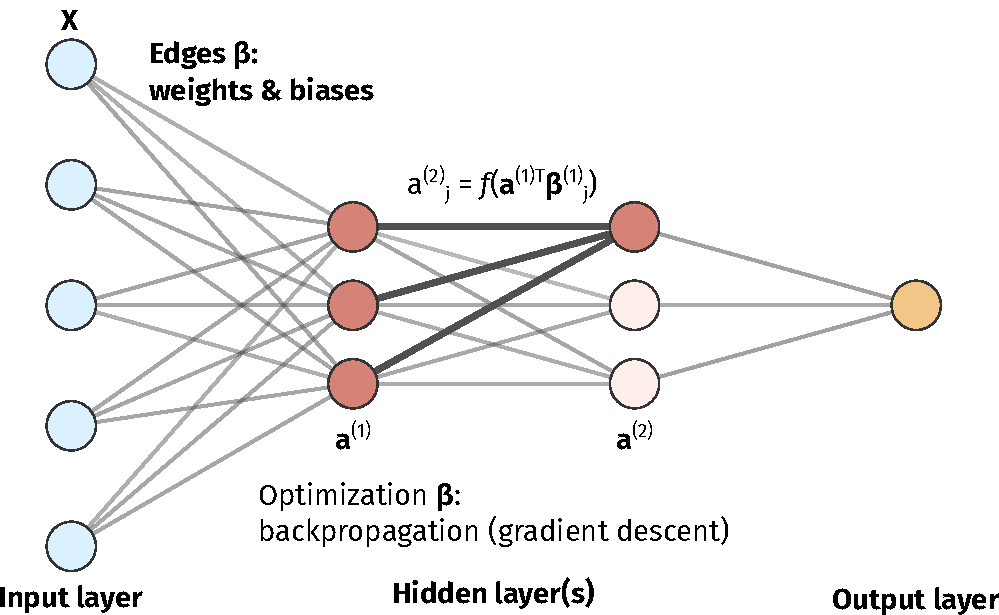
\includegraphics[width=0.85\linewidth]{images/nn-2.pdf}
        \end{figure}
        
      \end{frame}

      \begin{frame}
        \frametitle{Logistic Regression as Single-Node NN}
        Can single logistic neuron solve non-linear classification
        problem?
        \movie[loop]{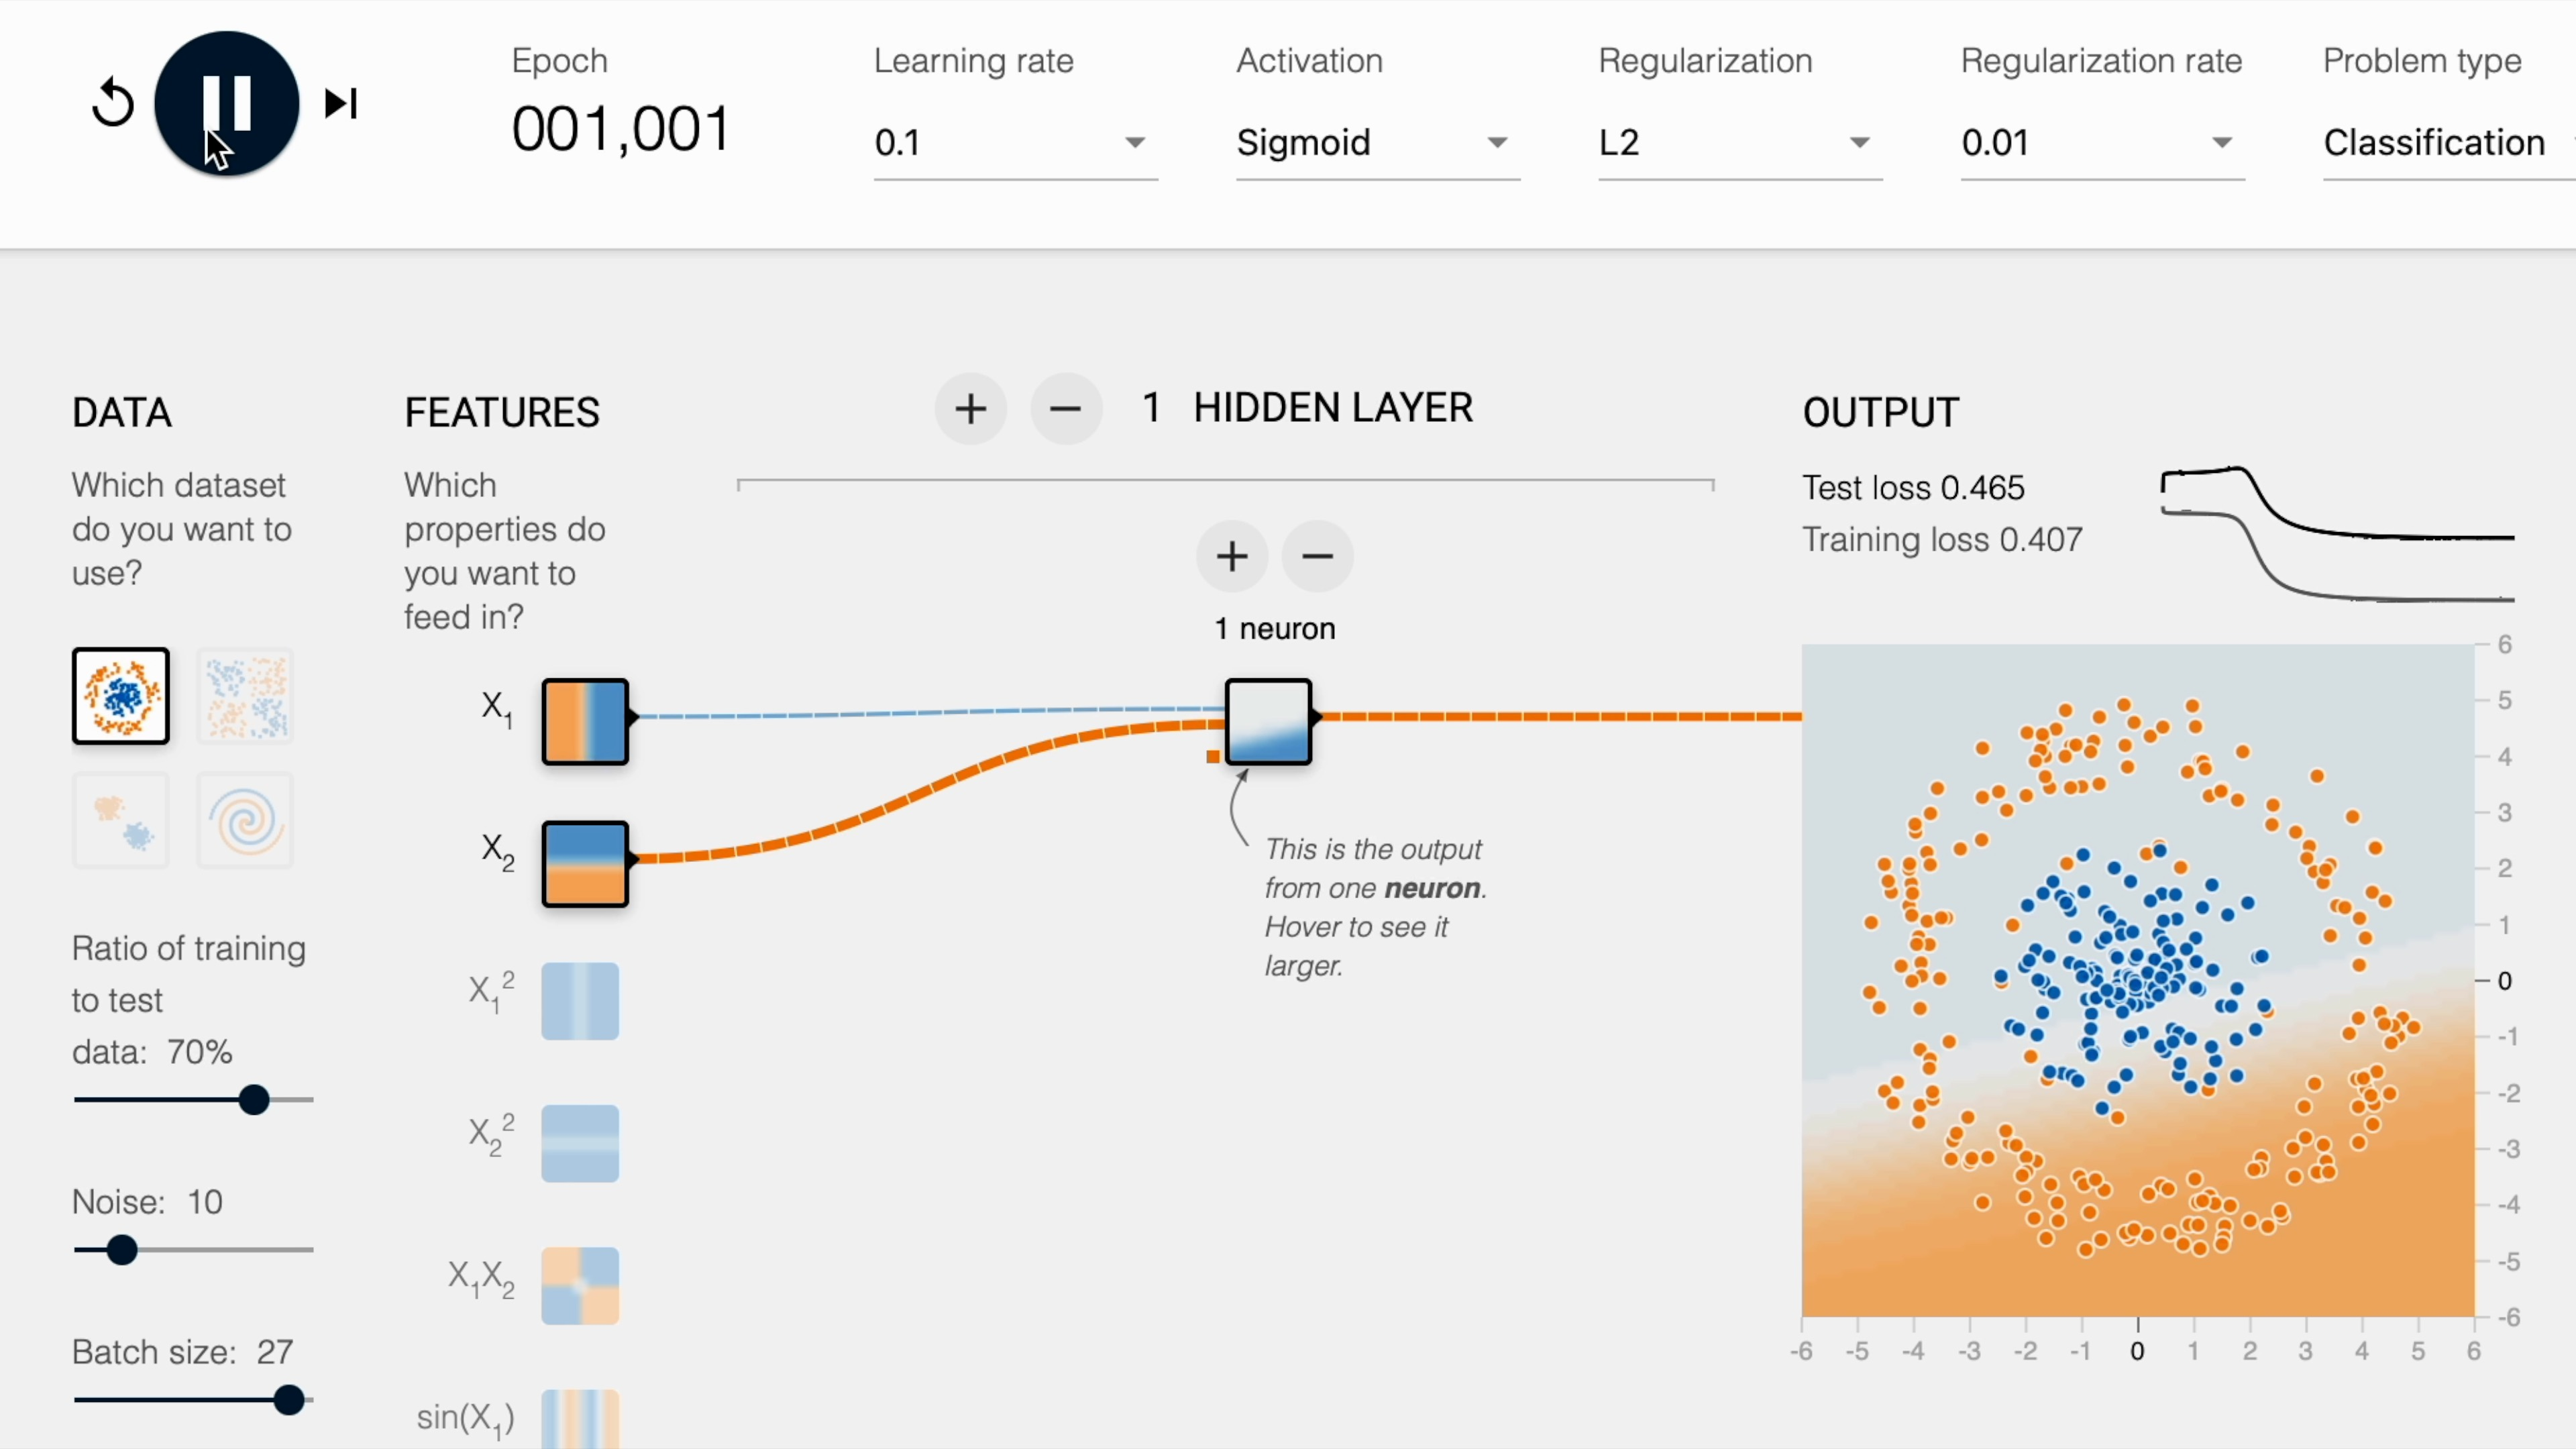
\includegraphics[width=0.90\textwidth]{images/nn-1-cover.jpg}}{images/nn-1-compressed.mov}
        \begin{tikzpicture}[remember picture, overlay]
          \node[anchor=north east, inner sep=1pt](image) at (current
          page.north east)
          {
\includegraphics[width=0.17\textwidth]{images/qr_1.png}};
          \node[anchor=north, align=center, inner sep=2pt] at
          (image.south) {Try it!};
        \end{tikzpicture}
        
      \end{frame}

      \begin{frame}
        \frametitle{Performance of Deeper NNs}
        Multi-neuron classification
        \movie[loop]{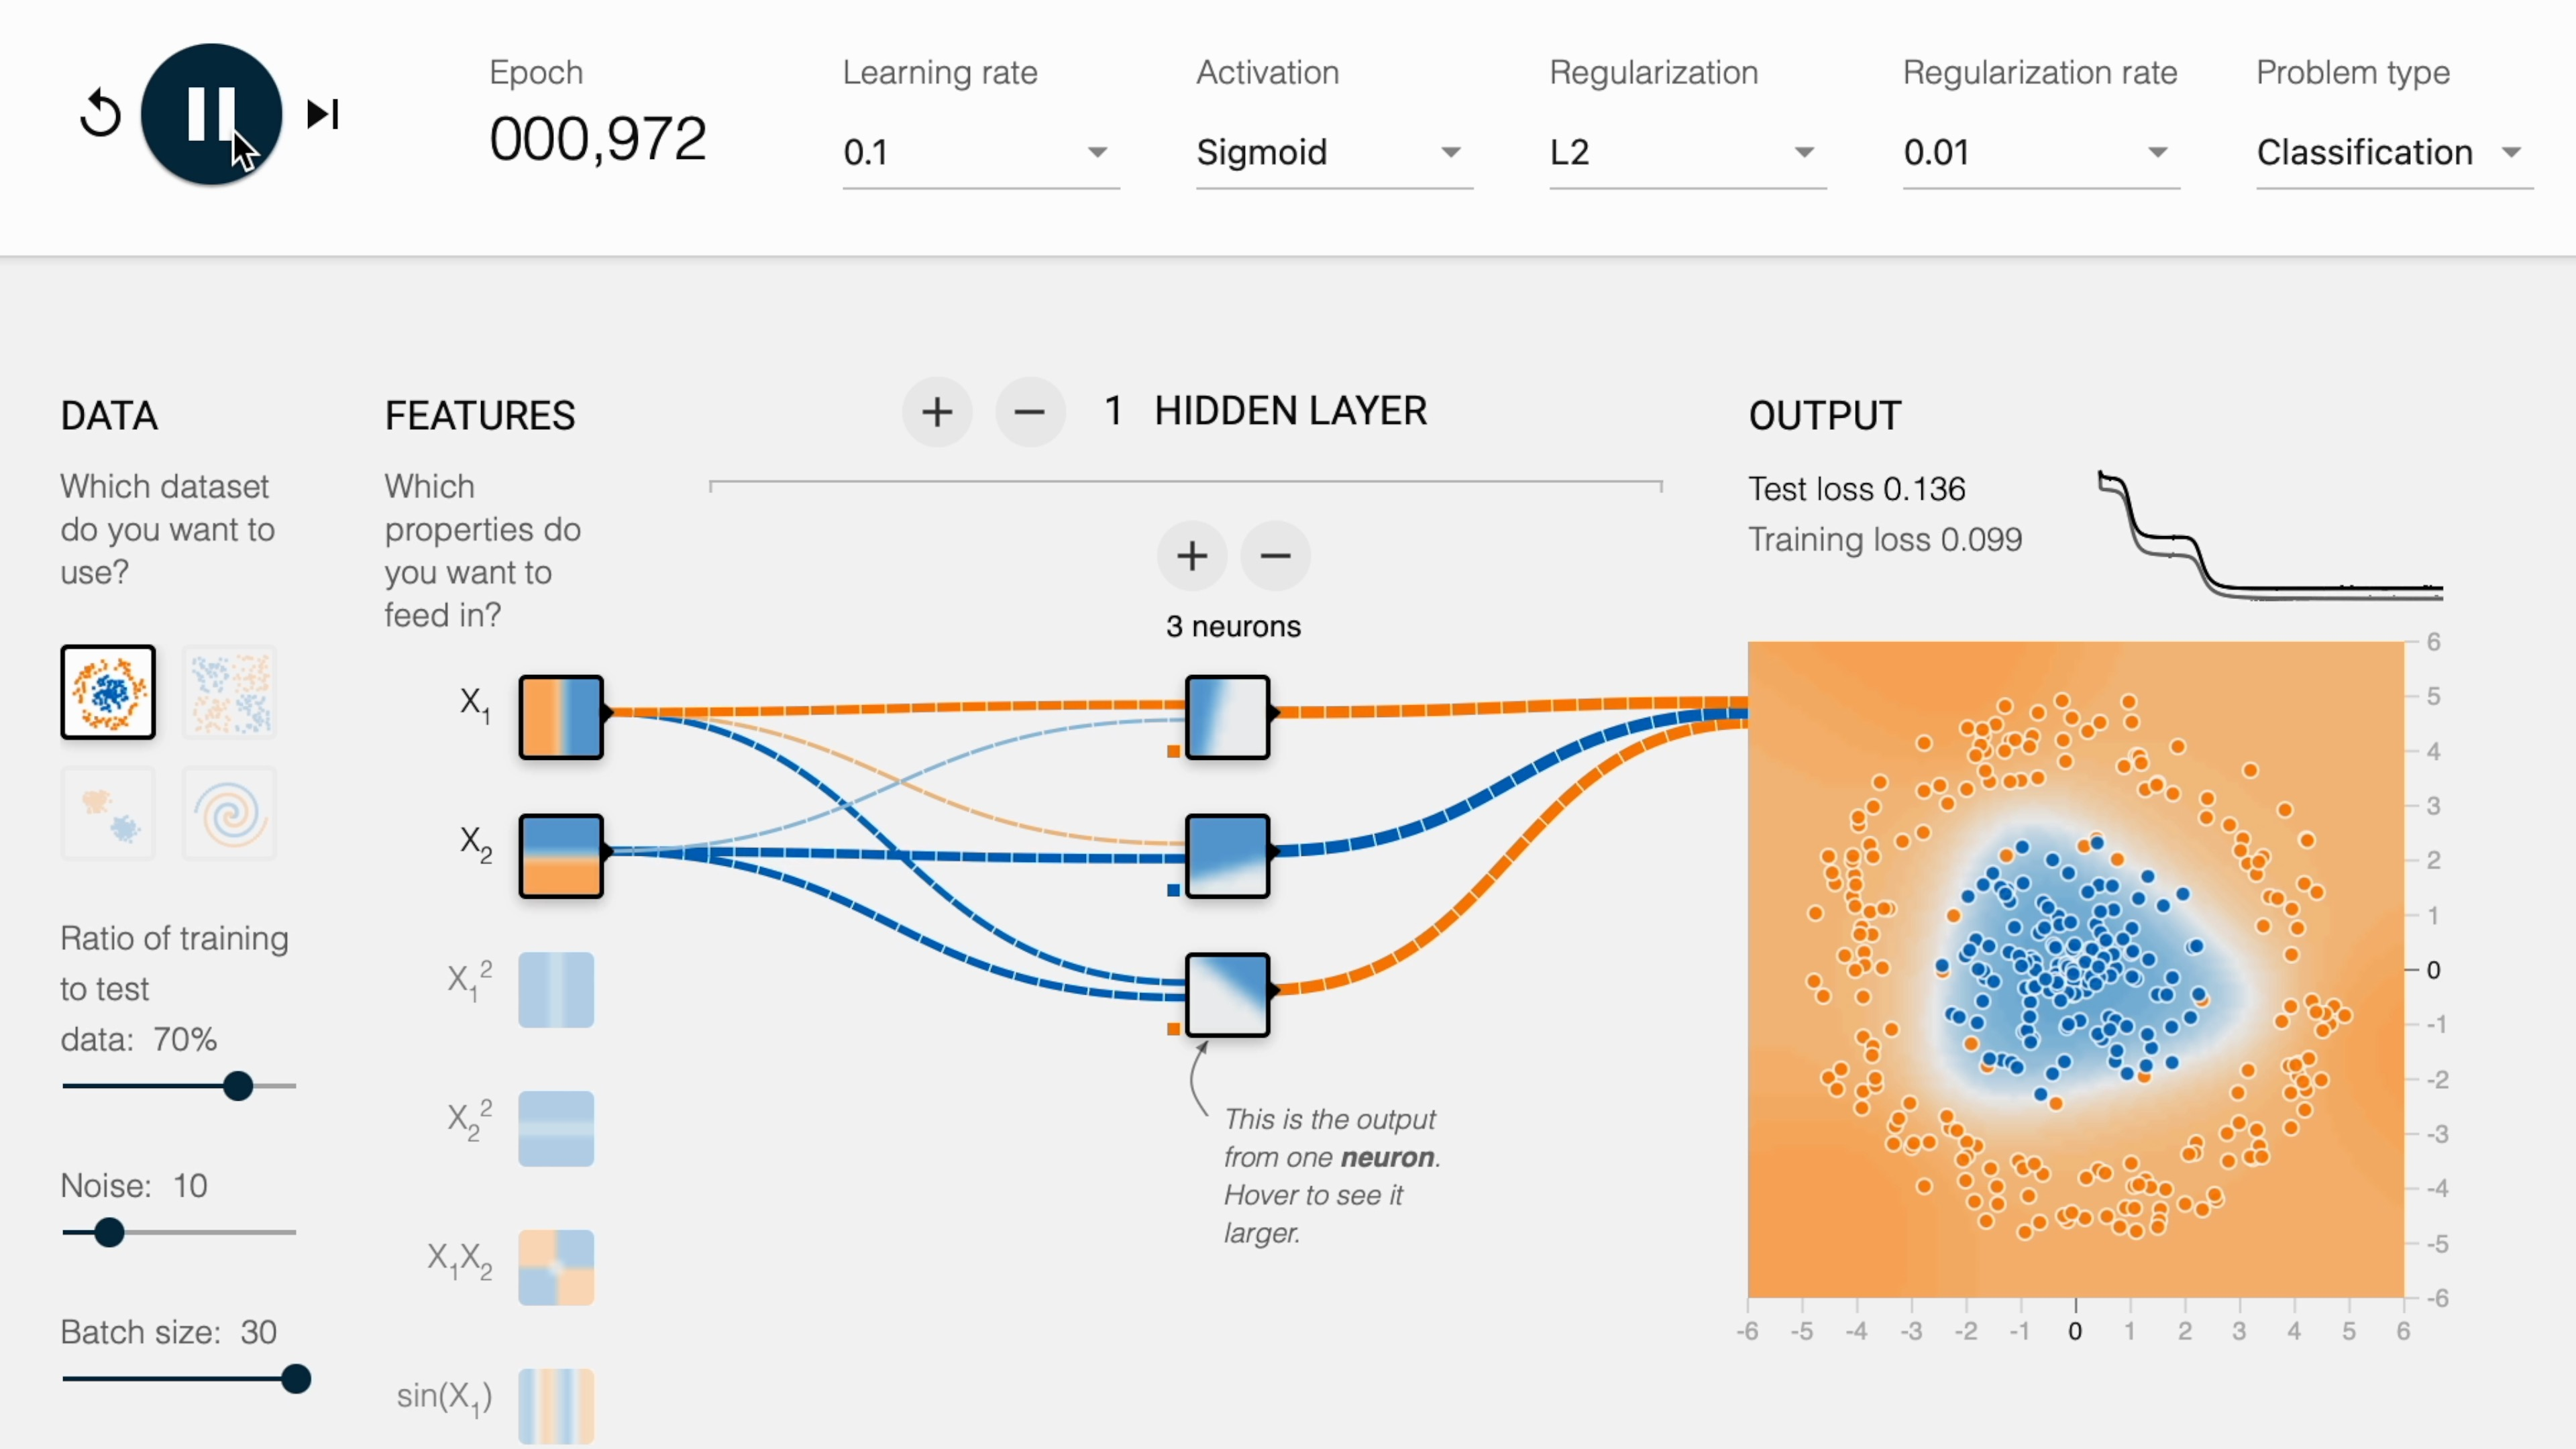
\includegraphics[width=0.90\textwidth]{images/nn-2-cover.jpg}}{images/nn-2-compressed.mov}
        \begin{tikzpicture}[remember picture, overlay]
          \node[anchor=north east, inner sep=1pt](image) at (current
          page.north east)
          {
\includegraphics[width=0.17\textwidth]{images/qr_2.png}};
          \node[anchor=north, align=center, inner sep=2pt] at
          (image.south) {Try it!};
        \end{tikzpicture}
      \end{frame}

      \begin{frame}
        \frametitle{Recap: Linear Regression vs Logistic Regression}
        \begin{columns}[T]
          \begin{column}{0.5\textwidth}
            \begin{minipage}[t][\textwidth][t]{1.0\linewidth}
              \textbf{Linear Regression}
              \begin{itemize}
                \vfill \item Model: $y = \beta_{0} + \beta_{1}x$
              
                \vfill \item Continuous response variable

              
                \vfill \item Linear relation between $x$ and $y$
              
                \vfill \item Fitting by minimizing least square error
              
                \vfill \item Model selection: maximizing $R^{2}$

              
                \vfill \item Reveal the trend in data
              \end{itemize}
            \end{minipage}
          \end{column}

          \begin{column}{0.5\textwidth}
            \begin{minipage}[t][\textwidth][t]{1.0\linewidth}
              \textbf{Logistic Regression}

              \begin{itemize}
                \vfill \item Model:
                $p =1 / (\exp[-(\beta_{0} + \beta_{1}x)]$

                \vfill \item Categorical response variable

                \vfill \item Linear between $x$ and $\log[p/(1-p)]$

                \vfill \item Fitting by maximizing likelihood

              
                \vfill \item Model selection: multiple metrics

              
                \vfill \item Classification \& probability estimation
              
              \end{itemize}
            \end{minipage}
          \end{column}
        \end{columns}
      \end{frame}

      \begin{frame}
        \frametitle{Open Questions}

        \begin{enumerate}
        \item Could you think of a way to extend binary logistic
          regression for multinomial classification problems?

          
        \item Could you prove that the logistic function's log-loss is
          a convex function?

          
        \item What if we use other sigmoid functions (e.g. scaled
          $\tanh$) for ``logistic'' regression? Could you compare the
          model robustness and computational expenses?
        
        \end{enumerate}
        
      \end{frame}

      \begin{frame}[c]
        \frametitle{}
        \centering \vspace{3em} {\Huge \bfseries Questions?}
      \end{frame}


      \begin{frame}
        \frametitle{Appendix: Visualize the Cost Function}
        Let's take a look at the cost function if there is only 1
        datum.
        
        \begin{columns}[T]
          \begin{column}{0.5\textwidth}
            \begin{equation*}
              y = 1
            \end{equation*}
            \vspace{-4em}
            \begin{figure}[t]
              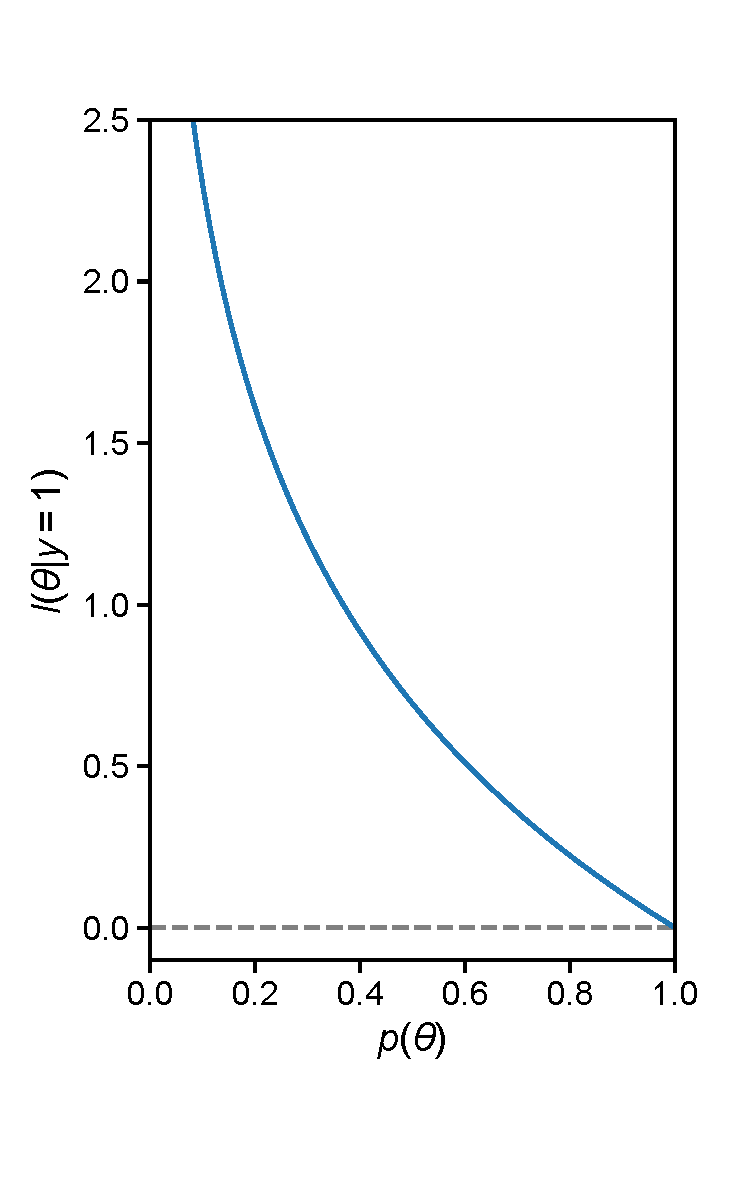
\includegraphics[width=0.75\textwidth]{scripts/loss_1.pdf}
            \end{figure}
          \end{column}

          \begin{column}{0.5\textwidth}
            \begin{equation*}
              y = 0
            \end{equation*}
            \vspace{-4em}
            \begin{figure}[t]
              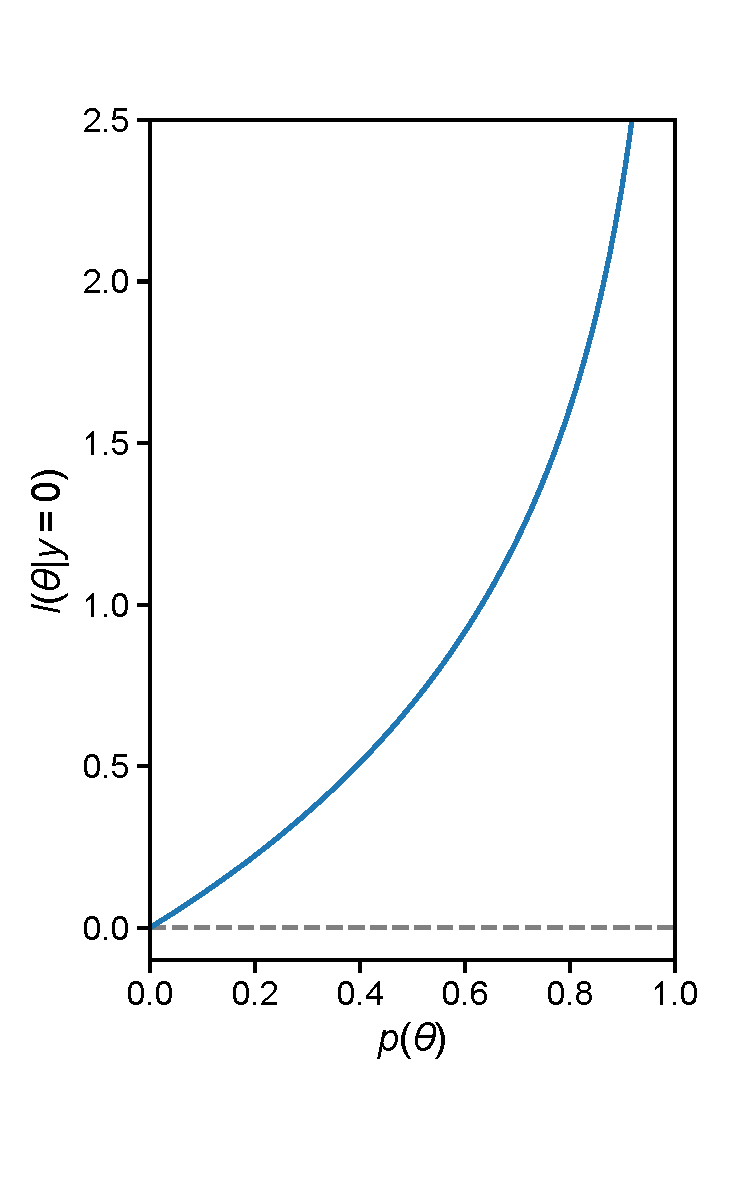
\includegraphics[width=0.75\textwidth]{scripts/loss_2.pdf}
            \end{figure}
          \end{column}
          
        \end{columns}
      \end{frame}

      \begin{frame}
        \frametitle{Visualize the Gradient Descent}

        In practice, many other methods like the
        Broyden–Fletcher–Goldfarb–Shanno (BFGS) algorithm have better
        performance than the Newton's method.

        \begin{figure}[t]
          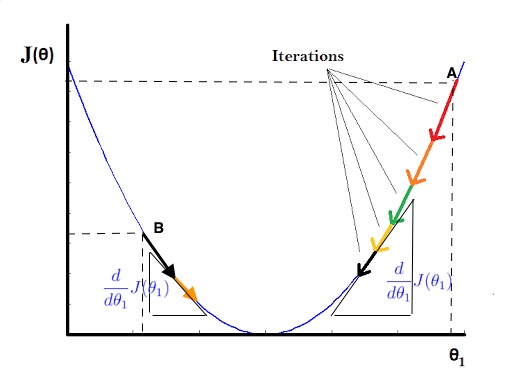
\includegraphics[width=0.5\textwidth]{images/gd-placeholder.jpg}
        \end{figure}
      \end{frame}

      \begin{frame}
        \frametitle{Continuous vs Categorical Data}
        In contrast, response variables suitable for linear regression
        are:
        \begin{itemize}
        \item Continuous and quantitative
        \item Ordering is meaningful
        \item Distance is meaningful
        \end{itemize}

      \end{frame}

      \begin{frame}
        \frametitle{The Classification Problem}

        Given:
        \begin{enumerate}
        \item Dataset:
          $D = \{(X_{1}, y_{1}), (X_{2},y_{2}), \cdots , (X_{n},
          y_{n})\}$
        \item Categorical response variable $y$: $y_{i} \in C$,
          $C = \{C_{1}, C_{2}, \cdots, C_{k}\}$
    
        \item Find optimal classifier function: $p(X; \theta)$ that
          predicts the category using parameter set $\theta$
        \end{enumerate}

        \vspace{2em}

        What a classification model will achieve:
        \begin{enumerate}
        \item Predict the categorical label
        \item Decision boundary for separation
        \item Probability of outcome
        \end{enumerate}
  
      \end{frame}

      \begin{frame}
        \frametitle{Solving Classification Problem by Regression}

        If the classifier function $p(X; \theta)$ corresponds to the
        \textbf{probability} of the outcome belonging to one class,
        the classification problem can be solved by regression.

        \vspace{2em}

  \begin{figure}[t]
    \vspace{-2em}
    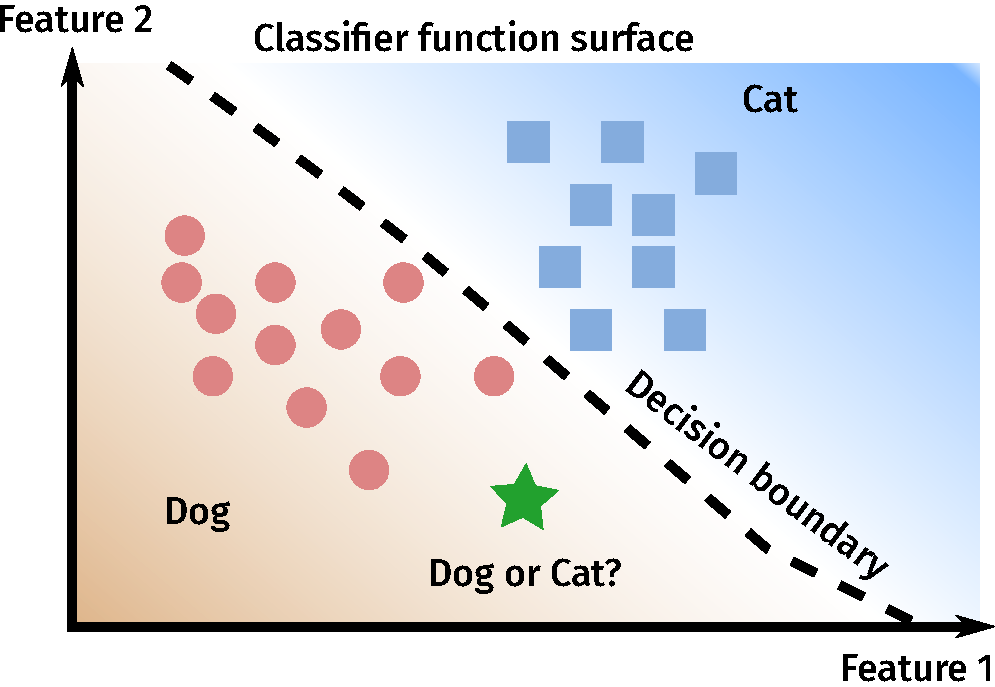
\includegraphics[width=0.6\textwidth]{images/classification_dog_cat.pdf}
  \end{figure}
  
\end{frame}
    
\end{document}
